\section{Concepts}
\label{chap2.section2}
Comme illustré dans "Figure \ref{fig:fig1}", le flux de travail\footnote{Un flux de travail est une série d'étapes impliquant des personnes et des systèmes qui sont effectuées afin d'atteindre un objectif au fil du temps. Autrement dit, c'est une succession de tâches qu'on effectue systematiquement pour faire un travail} typique d'un projet de science des données se compose de quatres grandes étapes:

\begin{enumerate}
    \item Organisation: La première étape consiste à organiser les données de sorte à formuler un problème précis qui implique souvent de prédire la valeur d'une variable ou de classifier les exemples en divers catégories. Durant cette étape nous collectons et organisons les tables qui nous intéresse à partir de diverses sources de données pour former un ensemble de données (\textbf{dataset})
    \item Interprêtation: Durant cette étape on analyse l'ensemble de données avec des programmes qui implémentent des méthodes statistiques d'agregation et de transformation afin de créer un ensemble de prédicateurs qui peuvent être utilisés pour distinguer ou predire la variable qui nous intéresse.
    \item Représentation: Durant cette étape nous cherchons à représenter les différentes variables sous une forme qui peut être comprise et manipulée par un ordinateur. Cela implique de représenter numériquement toutes les variables et de créer des tableaux, vecteurs ou matrices sur lesquels appliquer différents algorithmes et opérations mathématiques
    \item Apprentissage: Durant cette étape nous créons des modèles d'apprentissage automatique qui apprenent à interprêter les rélations entre les différentes variables afin de créer une approximation de la fonction inconnue qui a généré les données d'entraînement et enfin utiliser cette approximation pour prédire la variable dépendante.
\end{enumerate}

Dans les grands projets, ces différentes étapes sont typiquement exécutées par différentes personnes tous specialisé dans une des étapes. Un \textbf{Data Analyst} pour la première étape, un \textbf{Data Engineer} pour la séconde étape et un \textbf{Machine Learning Engineer} pour les deux dernières étapes. Un data scientist est une personne qui est capable d'exécuter le flux de travail de bout à bout, c'est-à-dire d'accomplir chacune de ces quatres étapes.

\begin{figure}
    \centering
    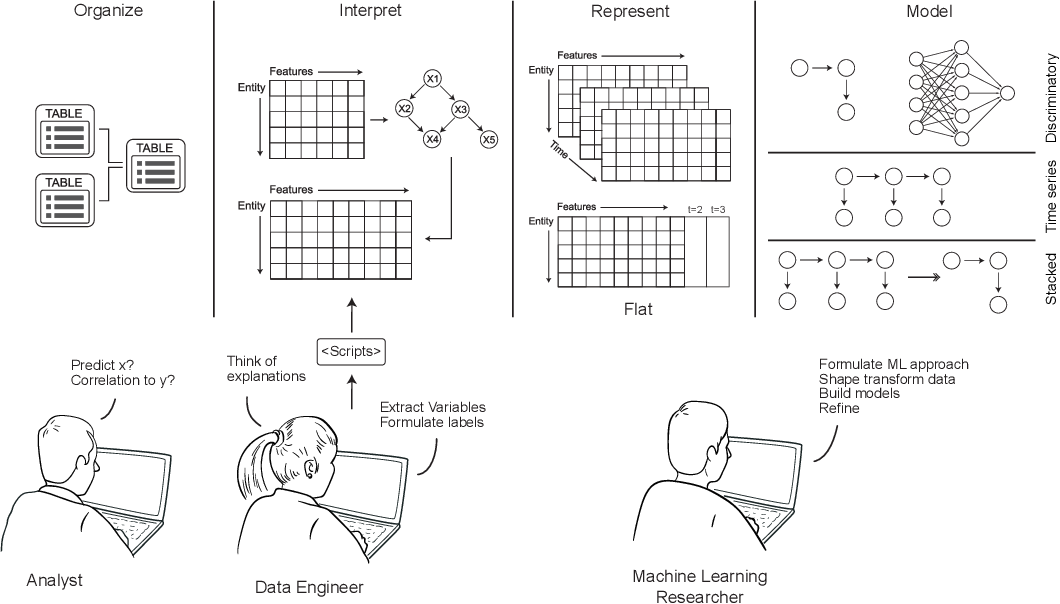
\includegraphics[width=0.75\linewidth]{images/Fig1DFS.png}
    \centering
    \caption{Le flux de travail d'un projet de science des données et les rôles impliqués}
    \label{fig:fig1}
\end{figure}

Dans mes recherches, j'ai exécuter ce flux de travail de la deuxième à la dernière étape, les données ayant déjà été collecter et organiser par Home Credit Group. Cela nécessite une connaissance des différents concepts impliqués dans chaque partie du flux de travail. La liste de définitions suivante couvre la plupart des notions fondamentales qui seront évoquées dans les prochains chapitres:

\begin{itemize}
    \item Une entité est une individualité possédant une existence et des caractéristiques propre. Dans ce document, une entité refère tout simplement à une table parmi celle de l'ensemble de données.
    \item Un prédicateur ou variable indépendante refère à une variable, une colonne dans une table pouvant être utiliser pour prédire une variable dépendante ou distinguer ces instances. Vous pourrez aussi entendre le mot anglais: \textbf{feature} pour faire référence à ce genre de variable. Par exemple la superficie d'une maison peut être utilisé pour prédire sa valeur.
    \item Une variable dépendante (\textbf{target}) est une variable/colonne dont on peut connaître la valeur en connaissant les valeurs d'une ou plusieurs variables indépendantes qui lui sont liées.
    \item Une instance est un cas particulier d'une entité où les différentes variables ou colonnes ont une valeur. On peut aussi parler d'exemple (eg: Un client, avec un nom, un genre, une addresse etc...).
    \item Une variable catégorique est un type de variable à valeur discrète et quantifiée (eg: La nationalité ou le sexe d'un client). À l'inverse une variable peut avoir des valeurs continues comme l'âge ou le salaire d'un client par exemple.
    \item La création ou l'ingenieurie de prédicateur est le processus qui permet de créer des variables indépendantes, généralement par aggrégation ou transformation de plusieurs variables de base.
    \item L'encodage est le processus par lequel on représente numériquement des variables qui ne sont pas de nature numérique (eg: sexe, ville...)
    \item Un entraînement réfère au processus lors duquel un model d'apprentissage automatique essaie de prédire la bonne valeur d'une variable dépendante pour tous les exemples d'un ensemble d'exemples d'entraînement dont on connait déjà la valeur de la variable dépendante, corrigeant ses erreurs grâce à un algorithme d'apprentissage.
    \item Un algorithme est une séquence d'instructions reproducible et de calculs mathématiques visant à résoudre un problème spécifique.
    \item Un pipeline: Ici le mot pipeline fait référence à l'implémentation d'un flux de travail, c'est un suite ordonnée d'étapes (pouvant inclure plusieurs algorithmes chacun) organisée de sorte à pouvoir exécuter entièrement ou partiellement un flux de travail.
\end{itemize}

Ce chapitre était un peu la condition pour que ce mémoire soit accessible à un plus grand nombre de personnes avec l'idée de diminuer au maximum les prérequis nécéssaire à la compréhension. Dans ce court chapitre j'ai surtout cherché à introduire quelques notions de base auxquels je ferai référence ou que je developperai dans les prochains chapitres afin de m'assurer que les lecteurs d'autres parcours ou d'autres domaines puisse suivre. Ceci conclut l'introduction, dans la partie méthodologie je rentre dans les détails des différents algorithmes et techniques de la science des données que j'ai utilisé lors de mes recherches et leur impléméntations.